\section{Implementation}

\subsection{Approach}

The \gls{good} model is implemented in Python using the Pyomo [SOURCE] and NetworkX [SOURCE] packages. The implementation leverages the specific capabilities of the mentioned packages. The \gls{good} model Operates on a power system represented as a directed graph using the NetworkX DiGraph class. The graph contains regions as nodes and transmission as edges. Nodes may contain an assets field which is a dictionary of assets. Policies are provided as a list. All nodes, edges, assets, and policies contain a dictionary of values used for object creation. 

The graph structure of the \gls{good} model is similar to other open-source Python power system modeling packages such as PyPSA [SOURCE] and SWITCH [SOURCE]. However, \gls{good}'s object structure differs substantially. On the back end, \textbf{PyPSA and SWITCH mimic the mathematical structure of the system}. These packages contain a centralized function for using the graph to build a model. \textbf{\gls{good} mimics the physical structure of the system}. After initiating an empty Pyomo model, \gls{good} passes the model to individual objects which modify and return it. This structure results in marginally slower build times but makes the package less opaque and extremely flexible. In the end, the package structure has no independent effect on solve times.

\subsection{Network Class}

The \gls{good} model starts with a Network object which takes global inputs, a power system graph, and a policy list as inputs as shown in Figure \ref{fig:network_class}.

\begin{figure}[H]
	\centering
	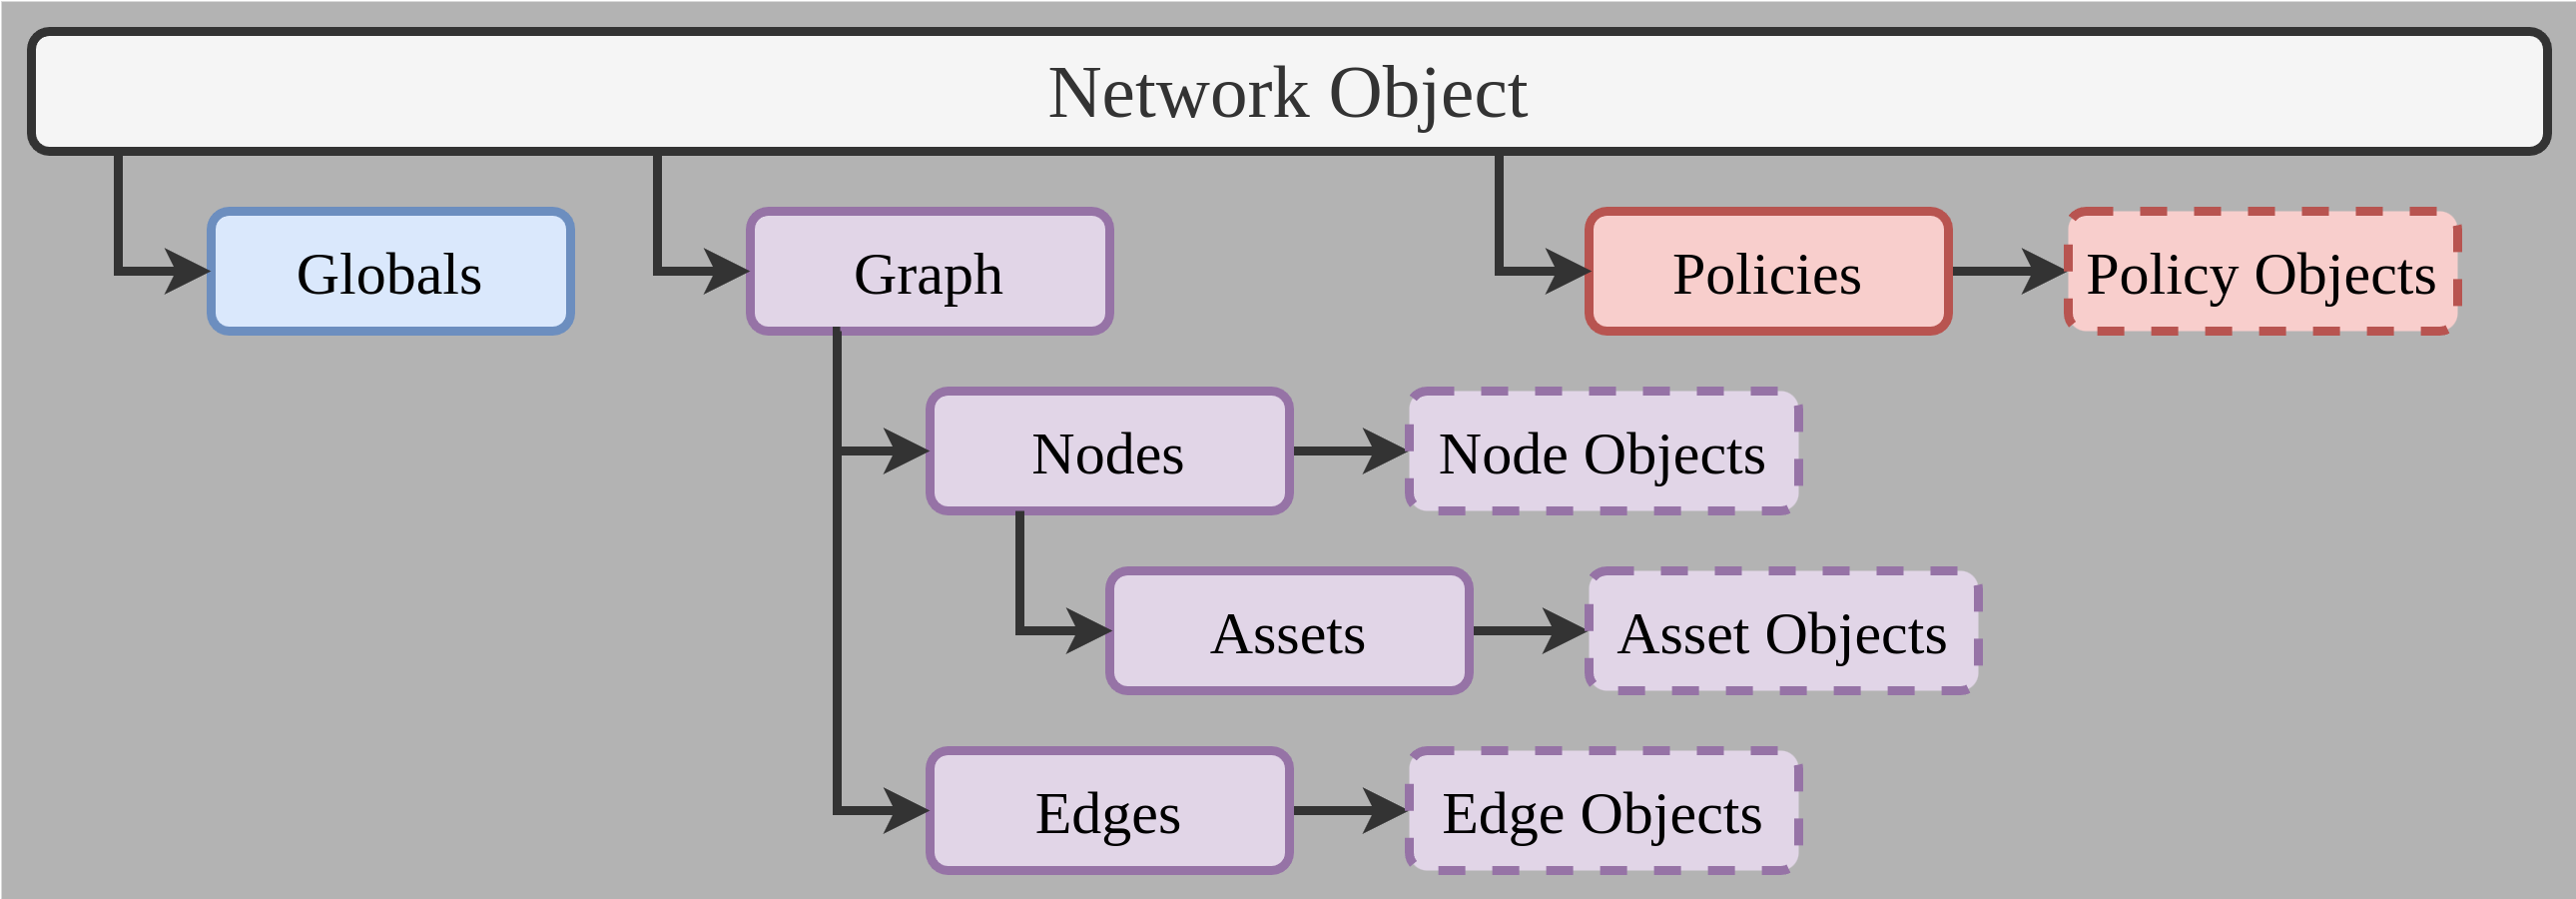
\includegraphics[width = \linewidth]{figs/network_class.png}
	\caption{Structure of the \gls{good} Network class. Dashed lines indicate \gls{good} objects.}
	\label{fig:network_class}
\end{figure}

The Network class has four functions:

\begin{enumerate}
	\item \textbf{Build Objects} - The Network object creates a \gls{good} object for each node, edge, asset, and policy and adds it to the appropriate element of the graph.
	\item \textbf{Build Model} - The Network object creates an empty Pyomo ConcreteModel then passes it to the \gls{good} objects to modify it.
	\item \textbf{Solve Model} - The complete model is solved using a Pyomo compatible solver.
	\item \textbf{Recover Results} - The Pyomo results are processed and added to the appropriate elements of the graph.
\end{enumerate}

\subsection{Element Base Classes}

\gls{good} represents a power system in terms of the following elements:

\begin{itemize}
	\item \textbf{Region}
	\item \textbf{Line}
	\item \textbf{RPS}
	\item \textbf{Load}
	\item \textbf{Producer}
	\item \textbf{Store}
\end{itemize}

There are four \gls{good} element base classes. The base classes are Node, Edge, Policy, and Asset. Base classes contain null versions of attributes which are required for model functionality. There are six default derived classes which inherit or modify the attributes of their base classes as shown in Figure \ref{fig:base_classes}.

\begin{figure}[H]
	\centering
	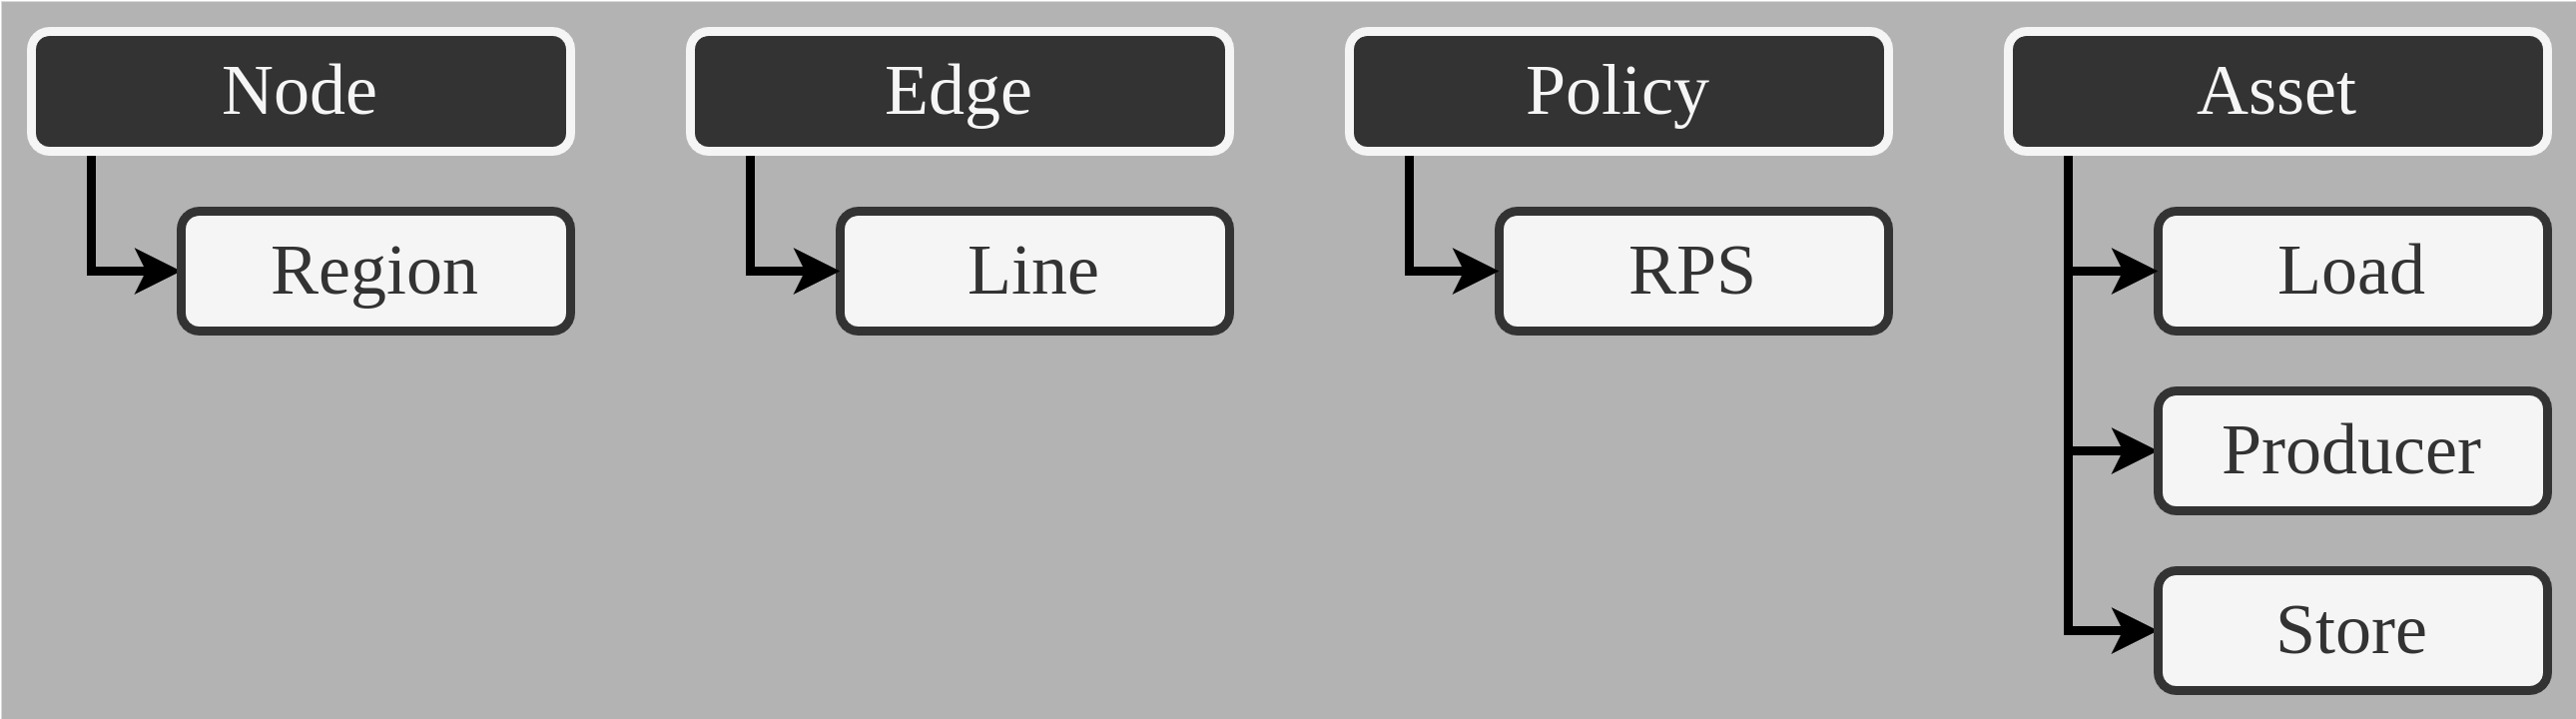
\includegraphics[width = \linewidth]{figs/base_classes.png}
	\caption{Base classes and derived classes.}
	\label{fig:base_classes}
\end{figure}

The primary purposes of \gls{good} objects are to modify the Pyomo ConcreteModel and process Pyomo results. Pyomo models can contain Pyomo set, parameter, variable, constraint, and objective objects. \gls{good} objects contain corresponding functions which take a model as input, add Pyomo objects to it, and return the modified model. These functions are referred to as "model-building" functions and are called for each object in a Network graph. The null version of a model-building function returns the model unmodified. Edge and Asset \gls{good} objects contain functions which are called by model-building functions. Finally, each \gls{good} object contains a results-recovery function which takes as input a solution graph and modifies and returns it. The functions of the element base classes are shown in Figure \ref{fig:base_class_functions}.

\begin{figure}[H]
	\centering
	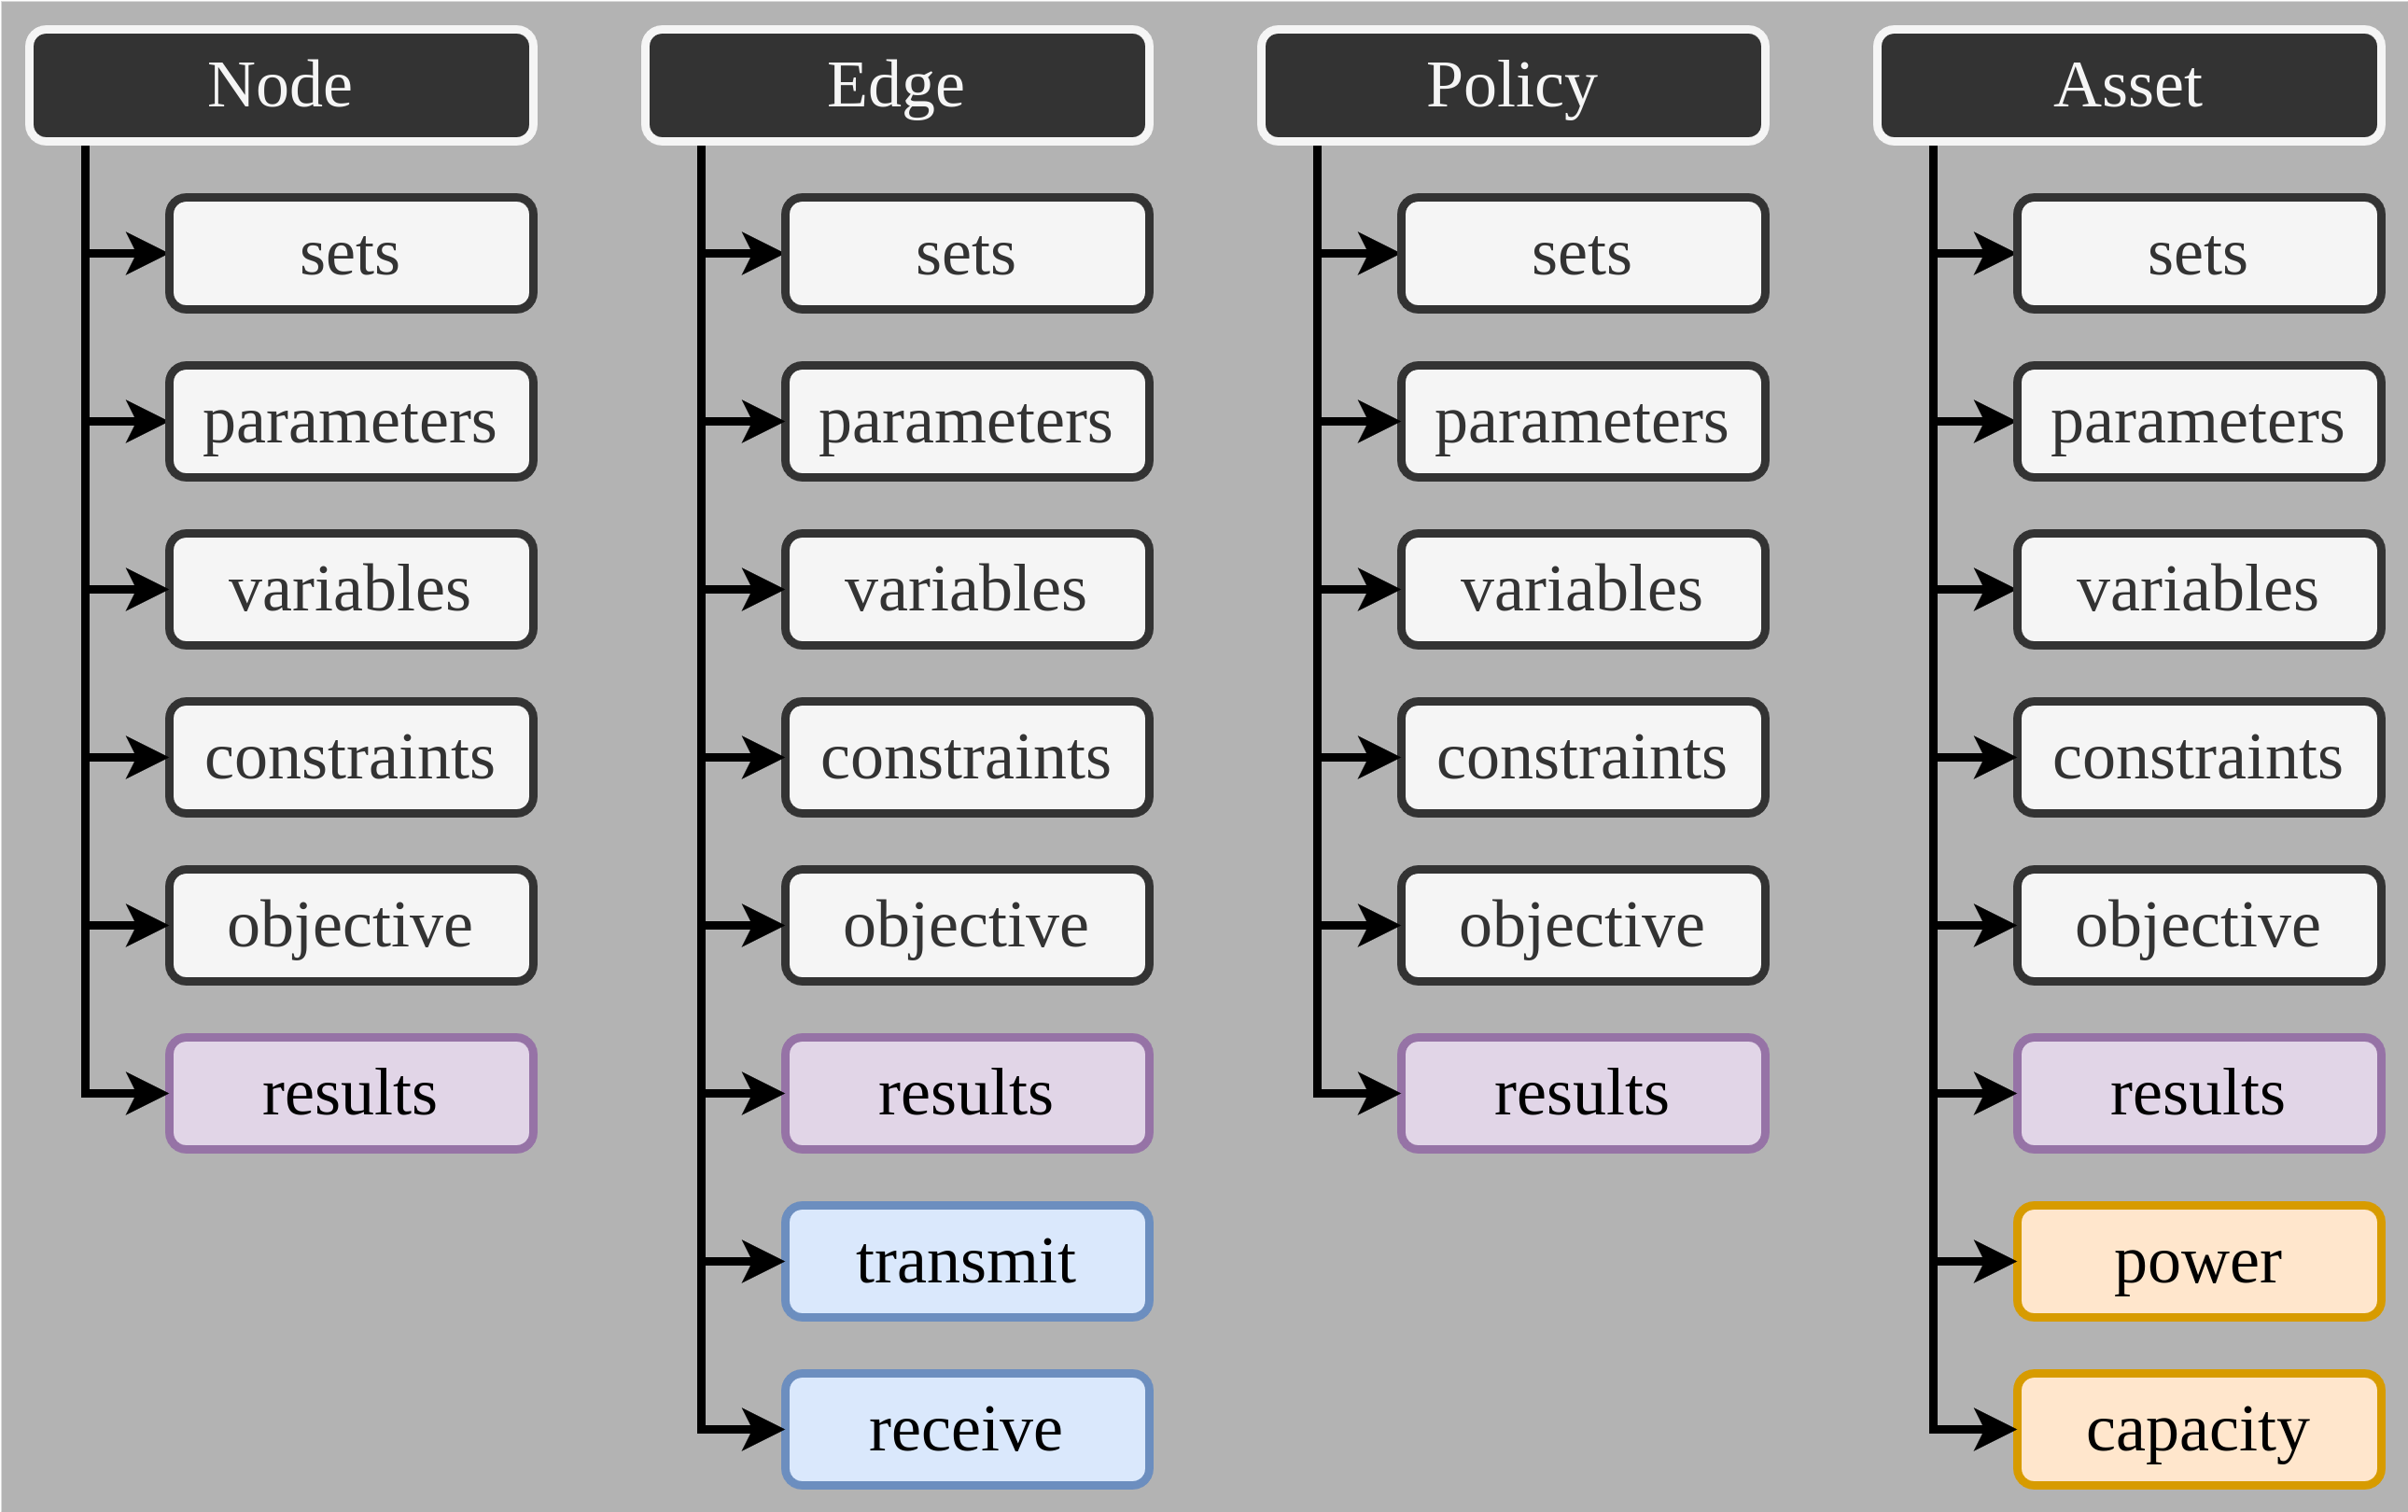
\includegraphics[width = \linewidth]{figs/base_class_functions.png}
	\caption{Base class functions. Light gray boxes are model-building functions and purple boxes are results-recovery functions.}
	\label{fig:base_class_functions}
\end{figure}